\chapter*{Introduction}
\addcontentsline{toc}{chapter}{Introduction}

\section*{What is \toolboxname?}
\addcontentsline{toc}{section}{What is \toolboxname?}

Lynx is a research-oriented Matlab toolbox for simulating in a fast way large machine learning experiments in the context of supervised and semi-supervised learning. To understand its goal, consider the following scenario: you, the researcher, have just developed a novel learning algorithm, commonly a variant of an already existing one. For simplicity, let us call them A and B. To test the efficacy of A involves comparing it against B (and possibly some additional baseline algorithms) on a large set of datasets. We call such a comparison a simulation. Results of a given simulation are then summarized and analyzed (maybe with the use of a statistical test) to understand relative strength and weaknesses of A with respect to B. Additionally, a simulation should be easily repeatable and modifiable, such that any other researcher employing similar tools can repeat it exactly or add its own additional features (e.g. another variant of B).

The converse situation is also typical: testing a large set of algorithms, possibly with different model selection strategies, on a particular dataset, to understand which one has the highest accuracy. Both settings become more complex if we possess more than a single machine, and we want to distribute the computational load among them, or if we are interested in speeding-up some of our computations using a GPU-based approach. This, together with the need of defining suitable strategies for subdividing data, and taking care that data itself is properly preprocessed, typically drive away the researcher from the high-level problems of the algorithm towards low-level, implementation-driven details.

\toolboxname is designed to handle both these situations using an high-level approach, taking charge of most part of the previously mentioned requirements in an automatic fashion. Hence, the user is left with the possibility of simply focusing on the elements of the simulation (e.g., which algorithms to include), and possibly on the details of a newly implemented feature. In particular, the user can specify the parameters of a simulation in a configuration file, which is then loaded by the software. The toolbox takes charge of importing the requested datasets, partitioning them, running the algorithms, collecting the results and analyzing them. It can distribute such simulations on multiple threads, and multiple computers, using the Parallel Computing Toolbox\footnote{\url{http://www.mathworks.it/products/parallel-computing/}} and the Distributed Computing Server\footnote{\url{http://www.mathworks.it/products/distriben/}} of Matlab. Moreover, many of the pre-implemented algorithms have the possibility of directly running on the GPU. The general schema of the toolbox is summarized in Fig. \ref{fig:generalschema}.

\begin{figure}
\centering
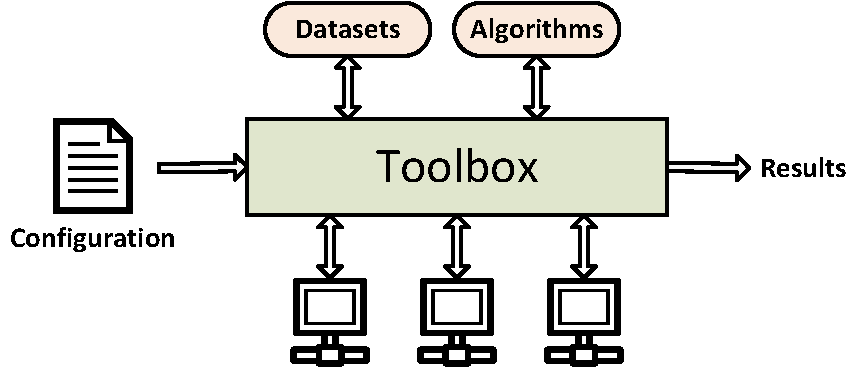
\includegraphics[scale=0.7]{./images/ToolboxSchema}
\caption{Schematic representation of the toolbox}
\label{fig:generalschema}
\end{figure}

At the end of any experiment, the toolbox provides information on the errors of each algorithm, their training times, and performs a statistical testing of the results (if possible). All the information can additionally be saved in a folder (including a full transcript of the simulation) or exported in the form of a pdf file. A wide set of datasets is already included in the library, and new ones can be added by storing them in a proper format.\footnote{Additional datasets can also be downloaded from the author’s webpage at \url{http://ispac.ing.uniroma1.it/scardapane/software/lynx/}.} Also, since the main core of the toolbox is fully object-oriented, additional algorithms and functionalities can be designed by simply extending specified classes, and are successively recognized automatically by the software.
 
\section*{Structure of this Document}
\addcontentsline{toc}{section}{Structure of this Document}

The rest of this guide is structured as follows. Chapter \ref{chap:firstuse} starts by showing how to install the toolbox, along with any optional library. To start familiarizing with the toolbox, a sample configuration file is provided with it. The second part of Chapter \ref{chap:firstuse} shows how to run it and analyzes briefly the behavior of the software. Then, Chapter \ref{chap:configfile} details the way in which a configuration file can be customized. Additional functionalities (e.g., saving the results) are explored successively in Chapter \ref{chap:additionalfeatures}. Finally, Chapter \ref{chap:newfunctionalities} explains the core classes of the software and how to add new algorithms and datasets to it.